\documentclass{article}
\usepackage[utf8]{inputenc}     
\usepackage[T1]{fontenc}        
\usepackage[brazilian]{babel}   
\usepackage[a4paper, margin=2.5cm]{geometry}
\usepackage{style}
\usepackage{pdfpages}

\usepackage{url, hyperref}
\usepackage{array}
\usepackage{paralist}
\usepackage{tabularx}
\usepackage[
	style=numeric,
	sorting=none,
	maxbibnames=10]{biblatex}
\addbibresource{ref.bib}
\bibliography{ref.bib}

\begin{document}

\begin{titlepage}
  \centering

  \vspace*{1cm}

  
\includegraphics[width=0.30\textwidth]{./HACKERSDOBEM.png}

  \vspace{1.8cm}

  {\Huge\bfseries Security Assessment Report\par}

  \vspace{0.4cm}

  {\Large Ataques de Força Bruta e Comprometimento de Credenciais\par}

  \vspace{2.5cm}

  \begin{flushleft}
    \large
    \textbf{Programa:} Hackers do Bem -- Especialização Red Team\\[0.3cm]
    \textbf{Módulo:} Módulo 03\\[0.3cm]
    \textbf{Projeto:} Aula 15 -- Escrita de Relatórios\\[0.3cm]
    \textbf{Analista:} Gabriel dos Santos Schmitz\\[0.3cm]
    \textbf{Data:} 19 de Junho de 2026
  \end{flushleft}

  \vfill

  \rule{\textwidth}{1pt}

  \vspace{0.5cm}

  \textbf{Resumo}

  \vspace{0.3cm}

  \parbox{0.85\textwidth}{
    Relatório de avaliação de segurança realizado em ambiente
    controlado de laboratório, abrangendo atividades de
    reconhecimento, enumeração de serviços, ataques de força
    bruta, comprometimento de credenciais, autenticação por
    chaves SSH e análise de impacto das vulnerabilidades
    identificadas.
  }

  \vspace{0.5cm}

  \rule{\textwidth}{1pt}

  \vfill

  \small
  Classificação: Uso Acadêmico \hfill Versão 1.0

  \vspace{0.2cm}

  Documento gerado em 19/06/2026

\end{titlepage}

\newpage
\section*{Controle do Documento}

\begin{table}[H]
\centering
\begin{tabular}{|l|l|}
\hline
Versão & 1.0 \\ \hline
Data & 19/06/2026 \\ \hline
Autor & Gabriel dos Santos Schmitz \\ \hline
Projeto & Aula 15 -- Escrita de Relatórios \\ \hline
Classificação & Uso Acadêmico \\ \hline
Status & Final \\ \hline
\end{tabular}
\end{table}
\tableofcontents
\listoffigures

\newpage
\section{Resumo Executivo}

\paragraph{}
Foi realizada uma avaliação prática de segurança em um ambiente de laboratório
com o objetivo de identificar vulnerabilidades relacionadas à exposição de
informações, uso inadequado de credenciais e mecanismos de autenticação.

\paragraph{}
Durante os testes foram identificadas falhas que permitiram a obtenção de
informações sensíveis, descoberta de credenciais válidas, acesso a serviços
internos e comprometimento de contas privilegiadas. As técnicas utilizadas
incluíram enumeração de diretórios web, ataques de força bruta, geração de
wordlists personalizadas, autenticação por chave SSH e quebra de hashes de
senhas.

\paragraph{}
Os resultados demonstram como pequenas exposições de informações podem ser
encadeadas por um atacante para ampliar progressivamente seu nível de acesso no
ambiente, culminando no comprometimento de contas com privilégios elevados.


\section{Escopo}

\paragraph{}
Os testes foram realizados exclusivamente nos sistemas disponibilizados no
ambiente de laboratório da disciplina, utilizando a máquina atacante para
executar as atividades de reconhecimento, enumeração e exploração.

\paragraph{}
Foram avaliados serviços web, FTP, SSH e mecanismos de autenticação presentes
no ambiente, conforme as atividades propostas durante a prática.

\section{Metodologia}

\paragraph{}
A metodologia adotada seguiu etapas semelhantes às utilizadas em avaliações de
segurança reais:

\begin{enumerate}
  \item Reconhecimento e enumeração de serviços;
  \item Descoberta de diretórios e conteúdos expostos;
  \item Coleta de informações públicas;
  \item Geração de wordlists direcionadas;
  \item Ataques de força bruta contra serviços de autenticação;
  \item Exploração de credenciais obtidas;
  \item Identificação de mecanismos de acesso privilegiado;
  \item Quebra de hashes de senhas.
\end{enumerate}

\section{Achados}

\subsection{Achado 01 -- Exposição de Conteúdo em Diretórios Públicos}

\textbf{Severidade: Média}

\paragraph{}
Durante a enumeração do servidor web foi identificado conteúdo acessível em
diretórios associados a usuários do sistema. As informações disponibilizadas
permitiram coletar dados relevantes sobre hábitos, interesses e possíveis
padrões utilizados pelo usuário.

\paragraph{}
Essas informações foram posteriormente utilizadas para construção de uma
wordlist personalizada empregada em ataques de autenticação.

\textbf{Impacto}

\begin{itemize}
  \item Exposição de informações sensíveis;
  \item Facilitação de ataques de engenharia social;
  \item Auxílio na criação de listas de senhas direcionadas.
\end{itemize}

\textbf{Recomendação}

\begin{itemize}
  \item Revisar conteúdos publicados em áreas públicas;
  \item Aplicar princípio do menor privilégio para acesso a arquivos;
  \item Realizar monitoramento de informações expostas externamente.
\end{itemize}

\subsection{Achado 02 -- Credenciais Fracas em Serviço FTP}

\textbf{Severidade: Alta}

\paragraph{}
A utilização de uma wordlist construída especificamente para o usuário alvo
permitiu a identificação de credenciais válidas por meio de ataque de força
bruta contra o serviço FTP.

\paragraph{}
Após a autenticação foi possível acessar arquivos privados armazenados na conta
comprometida.

\textbf{Impacto}

\begin{itemize}
  \item Acesso não autorizado a informações internas;
  \item Possibilidade de vazamento de dados;
  \item Facilitação de movimentação lateral.
\end{itemize}

\textbf{Recomendação}

\begin{itemize}
  \item Implementar políticas robustas de senha;
  \item Habilitar bloqueio de conta após tentativas falhas;
  \item Utilizar autenticação multifator quando possível.
\end{itemize}

\subsection{Achado 03 -- Exposição de Chave Privada SSH}

\textbf{Severidade: Crítica}

\paragraph{}
Durante a análise dos arquivos disponíveis via FTP foi encontrada uma chave
privada SSH pertencente a uma conta privilegiada do sistema.

\paragraph{}
Após identificar o usuário associado à chave, foi possível autenticar-se com
sucesso no serviço SSH e obter acesso privilegiado ao ambiente.

\paragraph{}
A Figura~\ref{fig:ssh-priv} apresenta evidência do acesso obtido.

\begin{figure}[H]
  \centering
  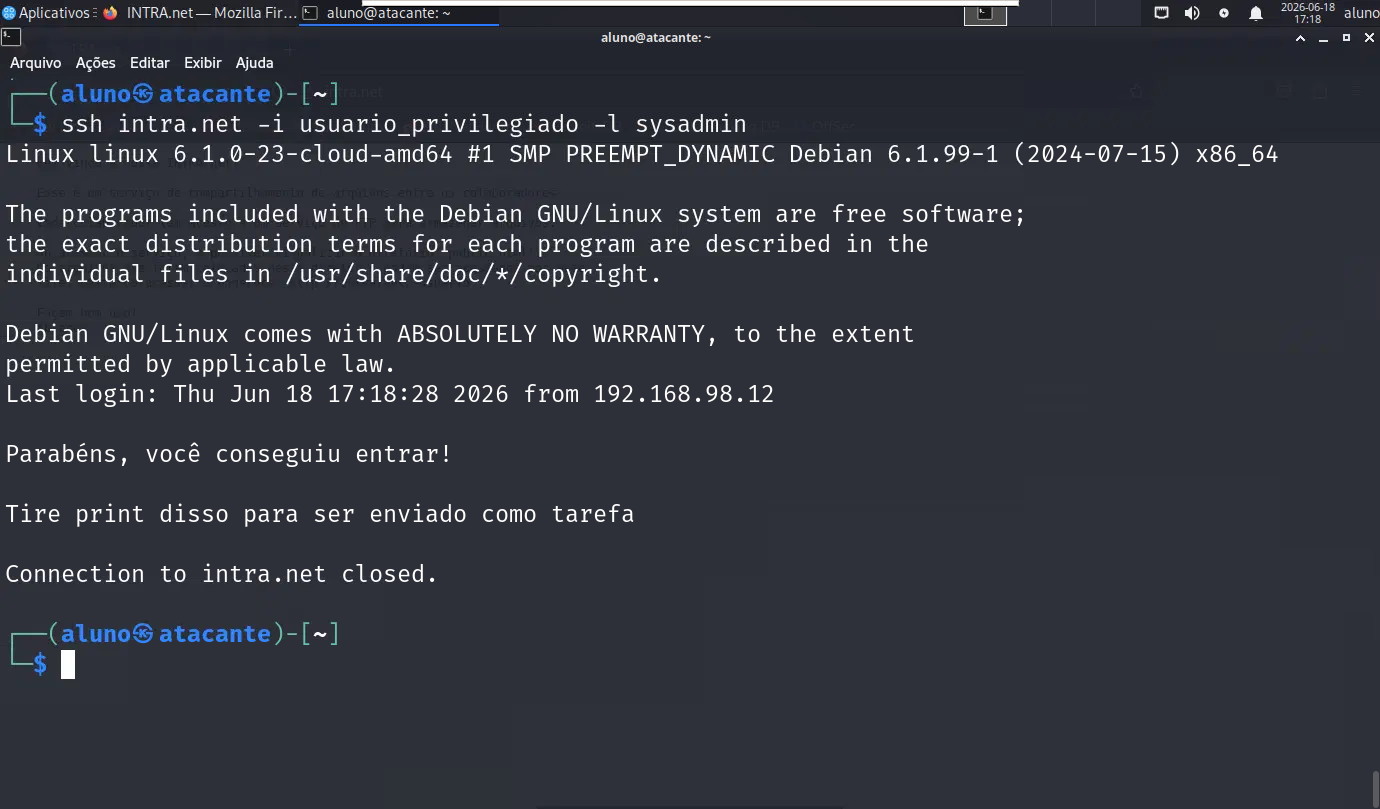
\includegraphics[width=0.95\textwidth]{./fig/login-ssh-privilegiado.png}
  \caption{Acesso SSH obtido utilizando chave privada exposta.}
  \label{fig:ssh-priv}
\end{figure}

\textbf{Impacto}

\begin{itemize}
  \item Comprometimento de conta privilegiada;
  \item Possibilidade de controle total do sistema;
  \item Acesso a informações sensíveis e recursos administrativos.
\end{itemize}

\textbf{Recomendação}

\begin{itemize}
  \item Armazenar chaves privadas de forma segura;
  \item Aplicar permissões restritivas aos arquivos sensíveis;
  \item Rotacionar imediatamente chaves expostas;
  \item Utilizar passphrase para proteção das chaves.
\end{itemize}

\subsection{Achado 04 -- Senha Previsível Baseada em Padrão Conhecido}

\textbf{Severidade: Média}

\paragraph{}
Foi identificado um padrão previsível na construção de senhas utilizado por um
usuário do ambiente.

\paragraph{}
A partir desse padrão foi criada uma expressão regular utilizada para gerar uma
wordlist direcionada. O conjunto reduzido de combinações permitiu identificar a
senha válida do usuário por meio de tentativa automatizada.

\textbf{Impacto}

\begin{itemize}
  \item Redução significativa do esforço necessário para ataques;
  \item Maior probabilidade de comprometimento de contas.
\end{itemize}

\textbf{Recomendação}

\begin{itemize}
  \item Utilizar senhas aleatórias;
  \item Evitar padrões previsíveis;
  \item Adotar gerenciadores de senha.
\end{itemize}

\subsection{Achado 05 -- Utilização de Hash MD5 para Armazenamento de Senhas}

\textbf{Severidade: Alta}

\paragraph{}
Foi identificado o uso do algoritmo MD5 para armazenamento de senhas.

\paragraph{}
As hashes obtidas foram submetidas ao processo de quebra utilizando a ferramenta
John the Ripper, resultando na recuperação das credenciais associadas.

\textbf{Impacto}

\begin{itemize}
  \item Comprometimento das credenciais armazenadas;
  \item Possibilidade de reutilização de senhas em outros sistemas;
  \item Aumento da superfície de ataque da organização.
\end{itemize}

\textbf{Recomendação}

\begin{itemize}
  \item Descontinuar o uso de MD5;
  \item Utilizar algoritmos modernos como Argon2, bcrypt ou scrypt;
  \item Implementar salting adequado nas senhas.
\end{itemize}

\section{Conclusão}

\paragraph{}
A avaliação demonstrou que múltiplas vulnerabilidades de baixa e média
complexidade podem ser combinadas para produzir impactos significativos na
segurança de um ambiente.

\paragraph{}
O processo iniciou com a simples enumeração de informações publicamente
acessíveis e evoluiu para comprometimento de credenciais, acesso a serviços
internos e obtenção de privilégios elevados por meio da exposição inadequada de
chaves SSH e utilização de mecanismos inseguros de armazenamento de senhas.

\paragraph{}
Os resultados reforçam a importância da adoção de boas práticas de segurança,
incluindo controle de exposição de informações, gerenciamento adequado de
credenciais, utilização de algoritmos modernos para proteção de senhas e
monitoramento contínuo dos ativos da organização.

\paragraph{}
A correção das vulnerabilidades identificadas reduz significativamente a
superfície de ataque e dificulta o encadeamento de técnicas que poderiam ser
utilizadas por agentes maliciosos para comprometer o ambiente.


\newpage
\printbibliography[title=Referências]

\end{document}
